\section{Modellering af PsykologNord og deres problemstilling}

Nu da der er en dybere forståelse for PsykologNord, deres problem og deres krav til løsningen, kan der kigges nærmere på, hvordan dette projekt har forsøgt at løse deres problemer.
Inden der skrives en masse kode er det dog nødvendigt at arbejde med deres problem og få det omdannet til modeller, som er nemmere at skrive et program ud fra.

Hvis man ikke har en ordenlig modellering af problemet vil det tage ekstra tid at levere en løsning, og kvaliteten af løsningen vil med stor sandsynlighed også være lavere.

Dette vil der blive arbejdet med i dette kapitel.

\subsection{Objektmodel}

For at have et værktøj til at skabe et overblik over virksomheden og dens gøremål, har vi lavet en objektmodel.
Modellen er lavet ud fra møderne med PsykologNord, og viden vi har tilegnet os om virksomheden gennem deres hjemmeside.\cite{psykolognord}

Objektmodellen, der kan ses på figur \ref{system:objekt} er udarbejdet med henblik på use casen ``Book Aftale'' beskrevet i afsnit \ref{usecase:bookaftale}.

Vi bruger objektmodellen til at hjælpe os med at visualisere hvilke ting fra PsykologNords hverdag, som vi skal have vores system til at indeholde og varetage.
Det er også et godt værktøj til at vise PsykologNord vores forståelse af deres arbejdsgang og virkelighed.

Objektmodellen er blevet opdateret hele vejen igennem forløbet, og den har været diskuteret igennem med vejledere og alle gruppens medlemmer flere gange.

Vores klientobjekt indeholder blandt andet et informationspunkt, der hedder journal.
Det har været diskuteret meget frem og tilbage i projektgruppen, om det skulle være sit ejet objekt eller ej.
Et argument for at have journalen som sit eget objekt vil være, at informationen i journalen bliver ændret uden at resten af klientobjektet ændres.
Vi har valgt at have det som et informationspunkt, da der altid vil være en en-til-en sammenhæng mellem en klient og en journal, og man derfor ikke kan have en journal uden en klient eller en klient uden en journal.

Aftale objektet er vores samleobjekt, da det binder de andre objekter sammen.

\begin{sidewaysfigure}
    \caption{Objektmodel for Book Aftale}
    \centering
        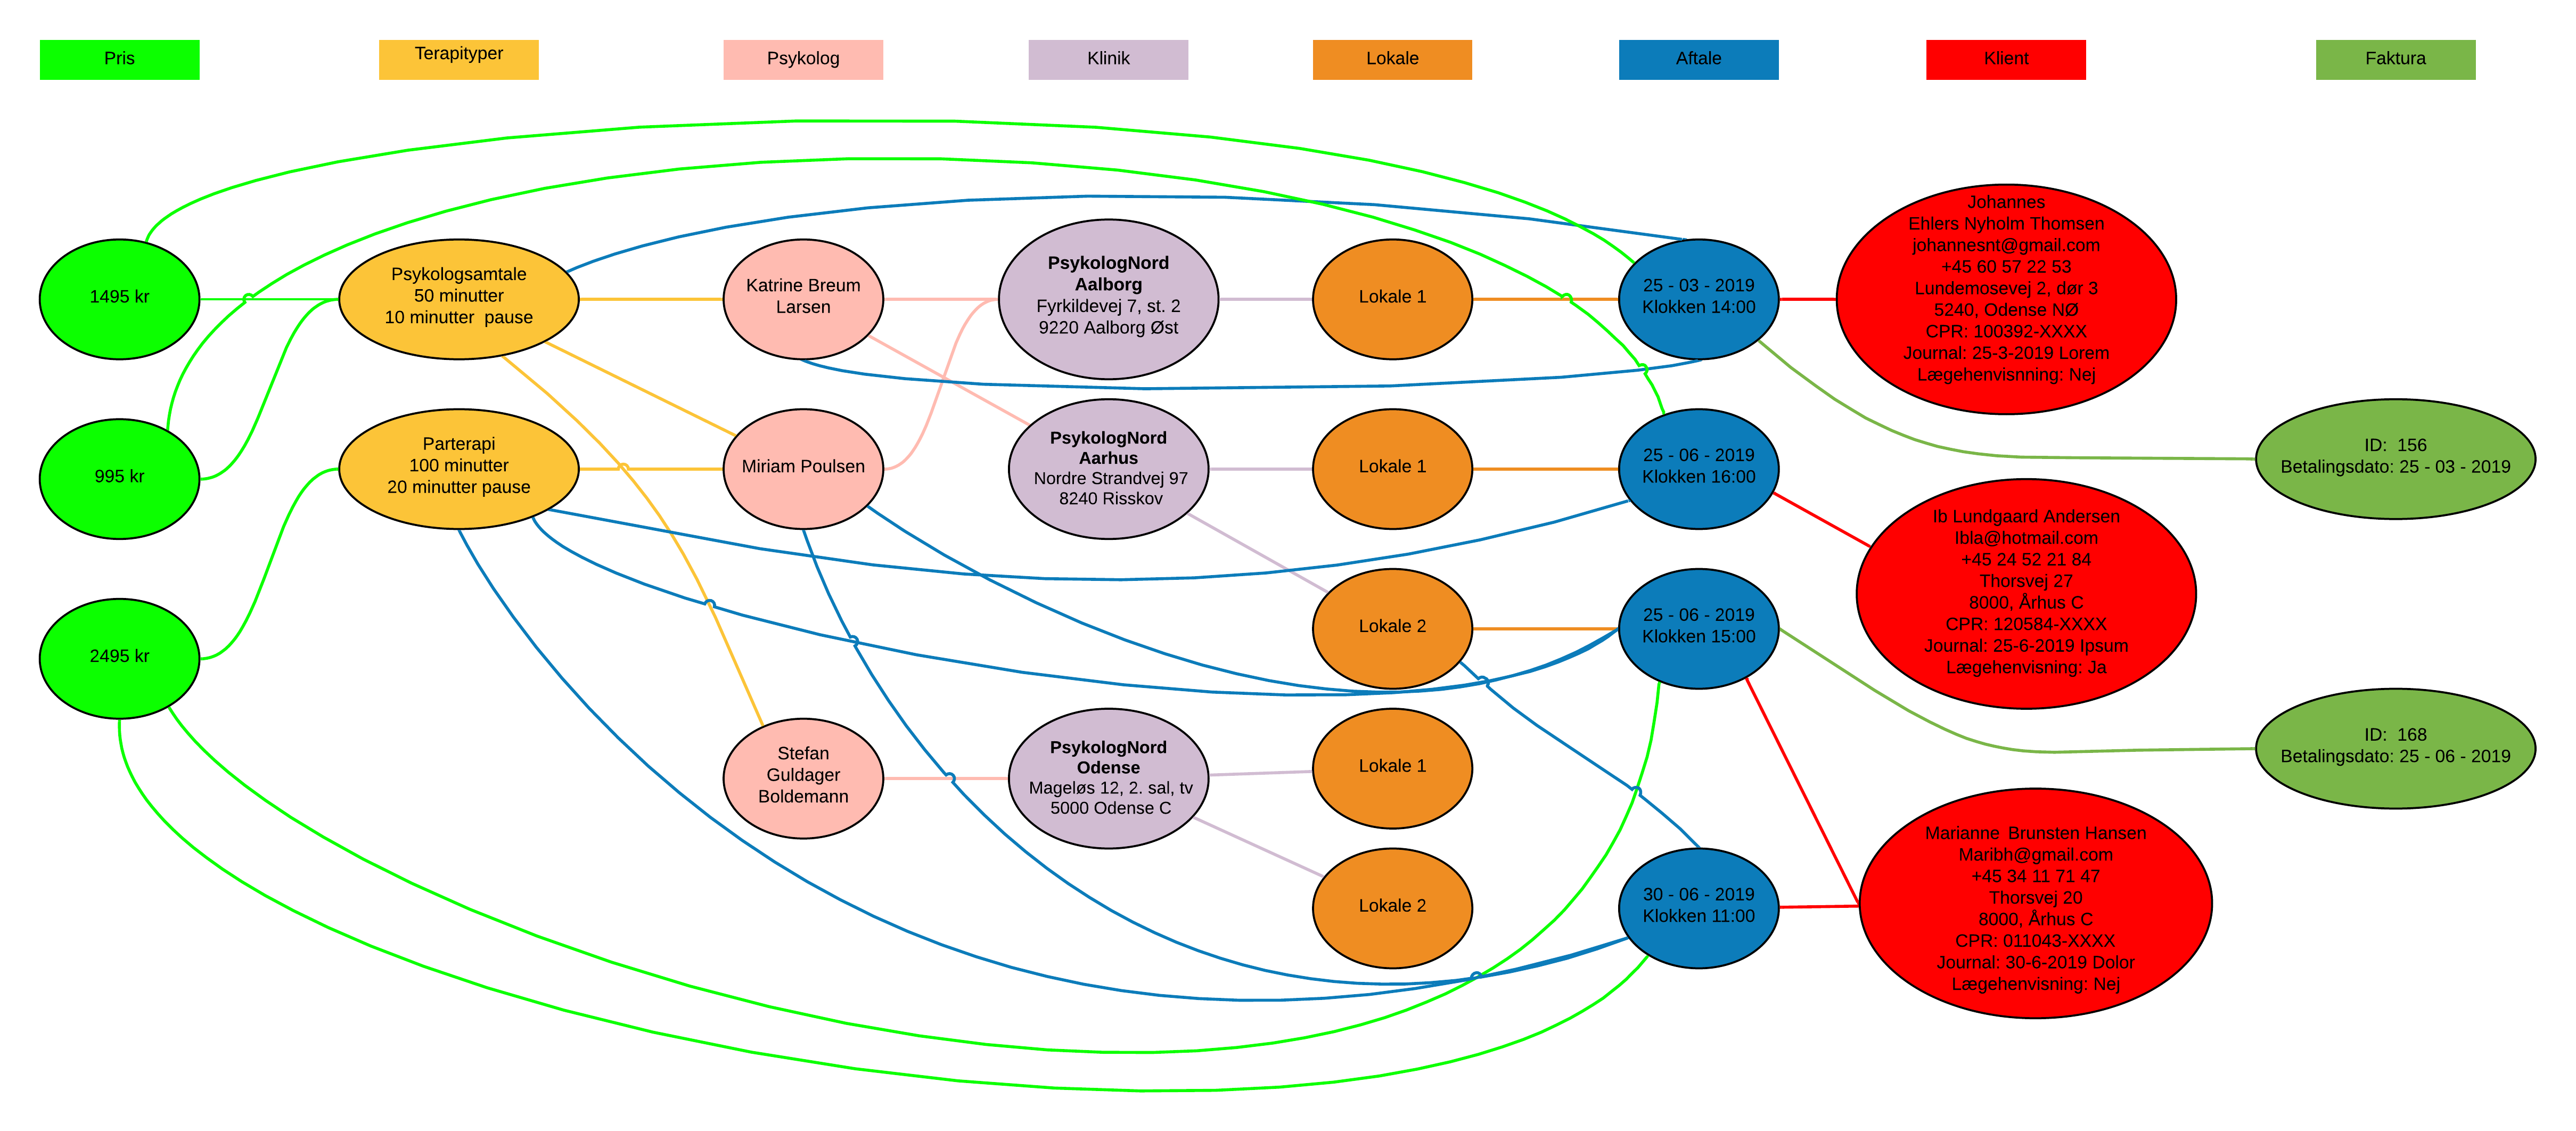
\includegraphics[width=\textwidth]{Objektmodel.png}
    \label{system:objekt}
\end{sidewaysfigure}

\subsection{Domænemodel}

På baggrund af objektmodellen kan vi så bygge videre til det næste artefakt, domænemodellen.
En domænemodel er en generalisering af objektmodellen.
Det er nødvendigt at lave en domænemodel, da en virksomhed ikke nødvendigvis er statisk.
Hvis man kun arbejder videre med en objektmodel modellerer man kun virkeligheden, som den er i det øjeblik, hvor modellen bliver konstrueret.
Så I vores tilfælde ville der bygges et system, som håndtere lige præcis de tre psykologer nævnt i objektmodellen, med lige præcis de terapityper, og så videre.
Men vi ved, at de har et ønske om at udvide, så derfor er det vigtigt at generalisere vores model, så den kan skaleres op og ned.

Domænemodellen bygges på de associationer og sammenhænge, som vi kan se i objektmodellen, f.eks kan vi se, at en aftale altid skal have mindst én klient, en klinik har et eller flere lokaler og så fremdeles.
Objekterne bliver oversat til domæneklasser, og deres sammenhænge bliver vist med associationer og kardinaliteter.

\begin{figure}[H]
    \caption{Domænemodel for Book Aftale}
    \centering
        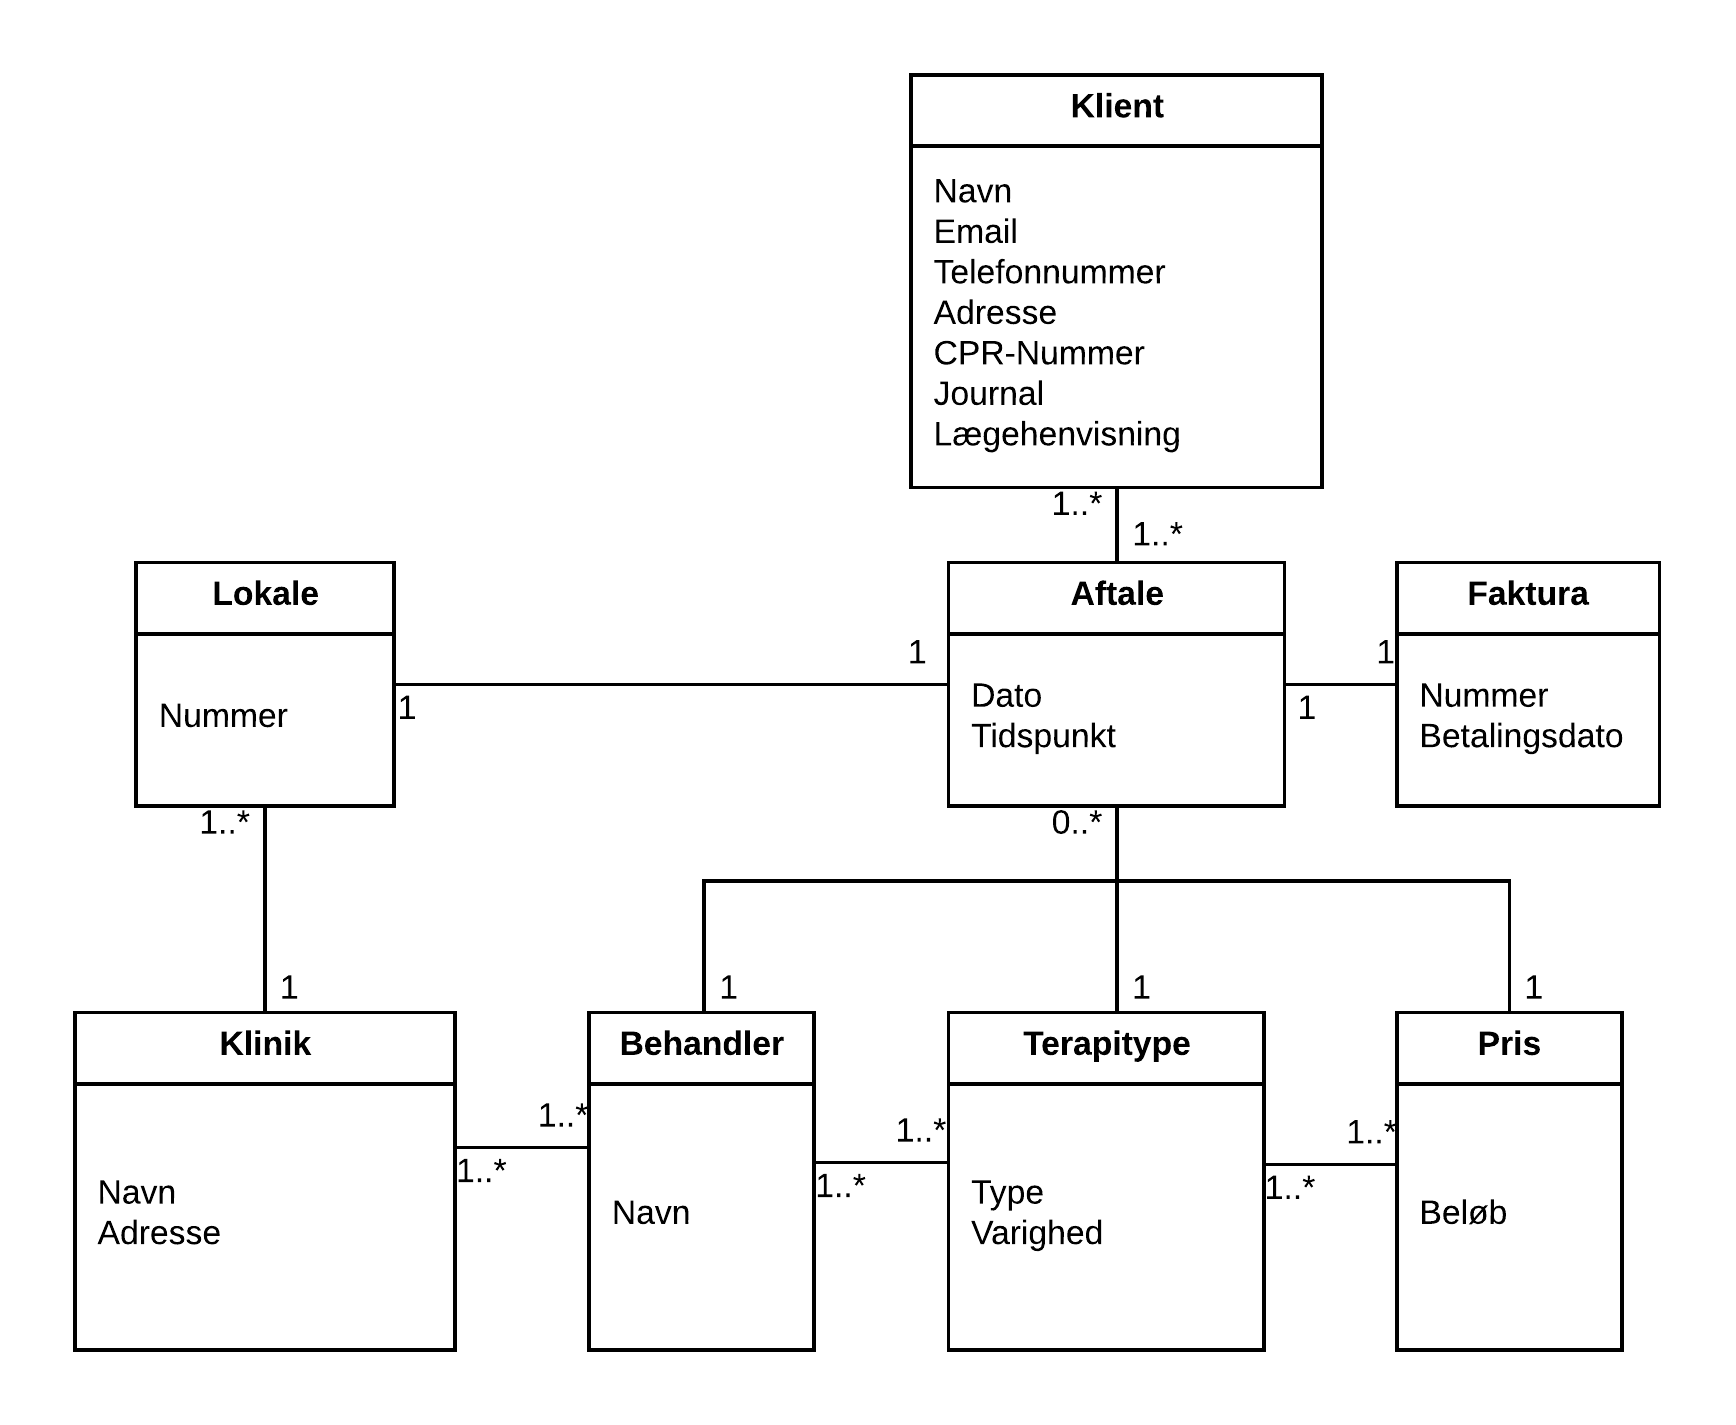
\includegraphics[width=\textwidth]{Domaenemodel.png}
    \label{system:domaene}
\end{figure}


